\PassOptionsToPackage{unicode=true}{hyperref} % options for packages loaded elsewhere
\PassOptionsToPackage{hyphens}{url}
\documentclass[11pt,ignorenonframetext,aspectratio=169]{beamer}
\IfFileExists{pgfpages.sty}{\usepackage{pgfpages}}{}
\setbeamertemplate{caption}[numbered]
\setbeamertemplate{caption label separator}{: }
\setbeamercolor{caption name}{fg=normal text.fg}
\beamertemplatenavigationsymbolsempty
\usepackage{lmodern}
\usepackage{amssymb,amsmath}
\usepackage{ifxetex,ifluatex}
\usepackage{fixltx2e} % provides \textsubscript
\ifnum 0\ifxetex 1\fi\ifluatex 1\fi=0 % if pdftex
  \usepackage[T1]{fontenc}
  \usepackage[utf8]{inputenc}
\else % if luatex or xelatex
  \ifxetex
    \usepackage{mathspec}
  \else
    \usepackage{fontspec}
\fi
\defaultfontfeatures{Ligatures=TeX,Scale=MatchLowercase}







\fi

  \usetheme[]{metropolis}






% use upquote if available, for straight quotes in verbatim environments
\IfFileExists{upquote.sty}{\usepackage{upquote}}{}
% use microtype if available
\IfFileExists{microtype.sty}{%
  \usepackage{microtype}
  \UseMicrotypeSet[protrusion]{basicmath} % disable protrusion for tt fonts
}{}


\newif\ifbibliography
  \usepackage[]{biblatex}
      \addbibresource{./../bibliography/bibliographies.bib}
  

\hypersetup{
      pdftitle={Probability and statistical testing},
        pdfauthor={Deependra Dhakal},
          pdfborder={0 0 0},
    breaklinks=true}
%\urlstyle{same}  % Use monospace font for urls







% Prevent slide breaks in the middle of a paragraph:
\widowpenalties 1 10000
\raggedbottom

  \AtBeginPart{
    \let\insertpartnumber\relax
    \let\partname\relax
    \frame{\partpage}
  }
  \AtBeginSection{
    \ifbibliography
    \else
      \let\insertsectionnumber\relax
      \let\sectionname\relax
      \frame{\sectionpage}
    \fi
  }
  \AtBeginSubsection{
    \let\insertsubsectionnumber\relax
    \let\subsectionname\relax
    \frame{\subsectionpage}
  }



\setlength{\parindent}{0pt}
\setlength{\parskip}{6pt plus 2pt minus 1pt}
\setlength{\emergencystretch}{3em}  % prevent overfull lines
\providecommand{\tightlist}{%
  \setlength{\itemsep}{0pt}\setlength{\parskip}{0pt}}

  \setcounter{secnumdepth}{0}


  \usepackage{setspace}
  \usepackage{wasysym}
  % \usepackage{fontenc}
  \usepackage{booktabs,siunitx}
  \usepackage{longtable}
  \usepackage{array}
  \usepackage{multirow}
  \usepackage{wrapfig}
  \usepackage{float}
  \usepackage{colortbl}
  \usepackage{pdflscape}
  \usepackage{tabu}
  \usepackage{threeparttable}
  \usepackage{threeparttablex}
  \usepackage[normalem]{ulem}
  \usepackage{makecell}
  \usepackage{xcolor}
  \usepackage{tikz} % required for image opacity change
  \usepackage[absolute,overlay]{textpos} % for text formatting
  \usepackage[skip=0.333\baselineskip]{caption}
  % \usepackage{newtxtext,newtxmath}% better than txfonts   
  \usepackage{tcolorbox}

  \sisetup{per-mode=symbol}

  % % Added by CII
  % \usepackage[format=hang,labelfont=bf,margin=0.5cm,justification=centering]{caption}
  % \captionsetup{font=small,width=0.9\linewidth,labelfont=small,textfont={small}}
  % % End of CII addition

  \usepackage{subcaption}
  % \newcommand{\subfloat}[2][need a sub-caption]{\subcaptionbox{#1}{#2}}

  \captionsetup[sub]{font=footnotesize,labelfont=footnotesize,textfont=footnotesize}
  % \captionsetup[subfigure]{font=small,labelfont=small,textfont=small}
  % \captionsetup[subfloat]{font=scriptsize,labelfont=scriptsize,textfont=scriptsize}

  % this font option is amenable for beamer, although these are global settings
  \setbeamerfont{caption}{size=\tiny}
  % \setbeamerfont{subcaption}{size=\tiny} % this does not chage subfloat fonts
  % \setbeamerfont{subfloat}{size=\tiny} % this does not change subfloat fonts
   
  % use single line spacing ?
  \singlespacing

  % use customize theme and colortheme
  % \usetheme[subsectionpage=progressbar,background=light]{metropolis}
  % \usetheme[]{Warsaw} % other options are: rose, Berlin
  % \usetheme[subsectionpage=progressbar,background=light]{metropolis} % it should be integrated to template itself by replacing preset theme
  \setbeamercolor{title}{fg=blue!85!black,bg=red!20!white}
  \setbeamertemplate{section in toc shaded}[default][50]
  % \usecolortheme{crane}
  \usecolortheme{seahorse}

  \newcommand{\bcolumns}{\begin{columns}[T, onlytextwidth]}
  \newcommand{\ecolumns}{\end{columns}}

  \newcommand{\bdescription}{\begin{description}}
  \newcommand{\edescription}{\end{description}}

  \newcommand{\bitemize}{\begin{itemize}}
  \newcommand{\eitemize}{\end{itemize}}

  % use cslreferences environment
  % this is revised as of Oct, 2022 (https://stackoverflow.com/questions/59193797/pandocs-environment-cslreferences-undefined-when-knitting-rmarkdown-to-pdf-in-r)
  \newlength{\cslhangindent}
  \setlength{\cslhangindent}{1.5em}
  \newenvironment{CSLReferences}%
    {\setlength{\parindent}{0pt}%
    \everypar{\setlength{\hangindent}{\cslhangindent}}\ignorespaces}%
    {\par}

  % % set option for tcolorbox
  % \tcbset{colback=red!5!white,colframe=red!75!black}
  % 
  % \setbeamertemplate{title page}{
  % 
  %         \begin{picture}(0,0)
  % 
  %             \put(85.33,-128){%
  %                 \pgfuseimage{mybackground}
  %             }
  % 
  %             \put(0,-110){%
  %                 \begin{minipage}[b][4cm][t]{13cm}
  %                     \raggedright
  %                     \begin{tcolorbox}[leftrule=2mm]
  %                     \usebeamerfont{title}{\inserttitle\par}
  %                     \end{tcolorbox}
  %                     \bigskip
  %                     \usebeamerfont{author}\insertauthor\par
  %                     \bigskip
  %                     \usebeamerfont{institute}\insertinstitute\par
  %                 \end{minipage}
  %             }
  % 
  %             \end{picture}
  % 
  %     }
  \usepackage{epsdice}

  \title[]{Probability and statistical testing}


  \author[
        Deependra Dhakal
    ]{Deependra Dhakal}

  \institute[
    ]{
    Agriculture and Forestry University\\
\textit{ddhakal.rookie@gmail.com}\\
\url{https://rookie.rbind.io}
    }

\date[
      Academic year: 2022-2023
  ]{
      Academic year: 2022-2023
        }


\begin{document}

% Hide progress bar and footline on titlepage
  \begin{frame}[plain]
  \titlepage
  \end{frame}



\hypertarget{the-probability-rules}{%
\section{The probability rules}\label{the-probability-rules}}

\begin{frame}{Probability}
\protect\hypertarget{probability}{}
\begin{columns}[T,onlytextwidth]
\column{0.5\textwidth}



\includegraphics[width=0.95\linewidth]{../images/fifty_percent_of_roger_federer} 

\column{0.5\textwidth}


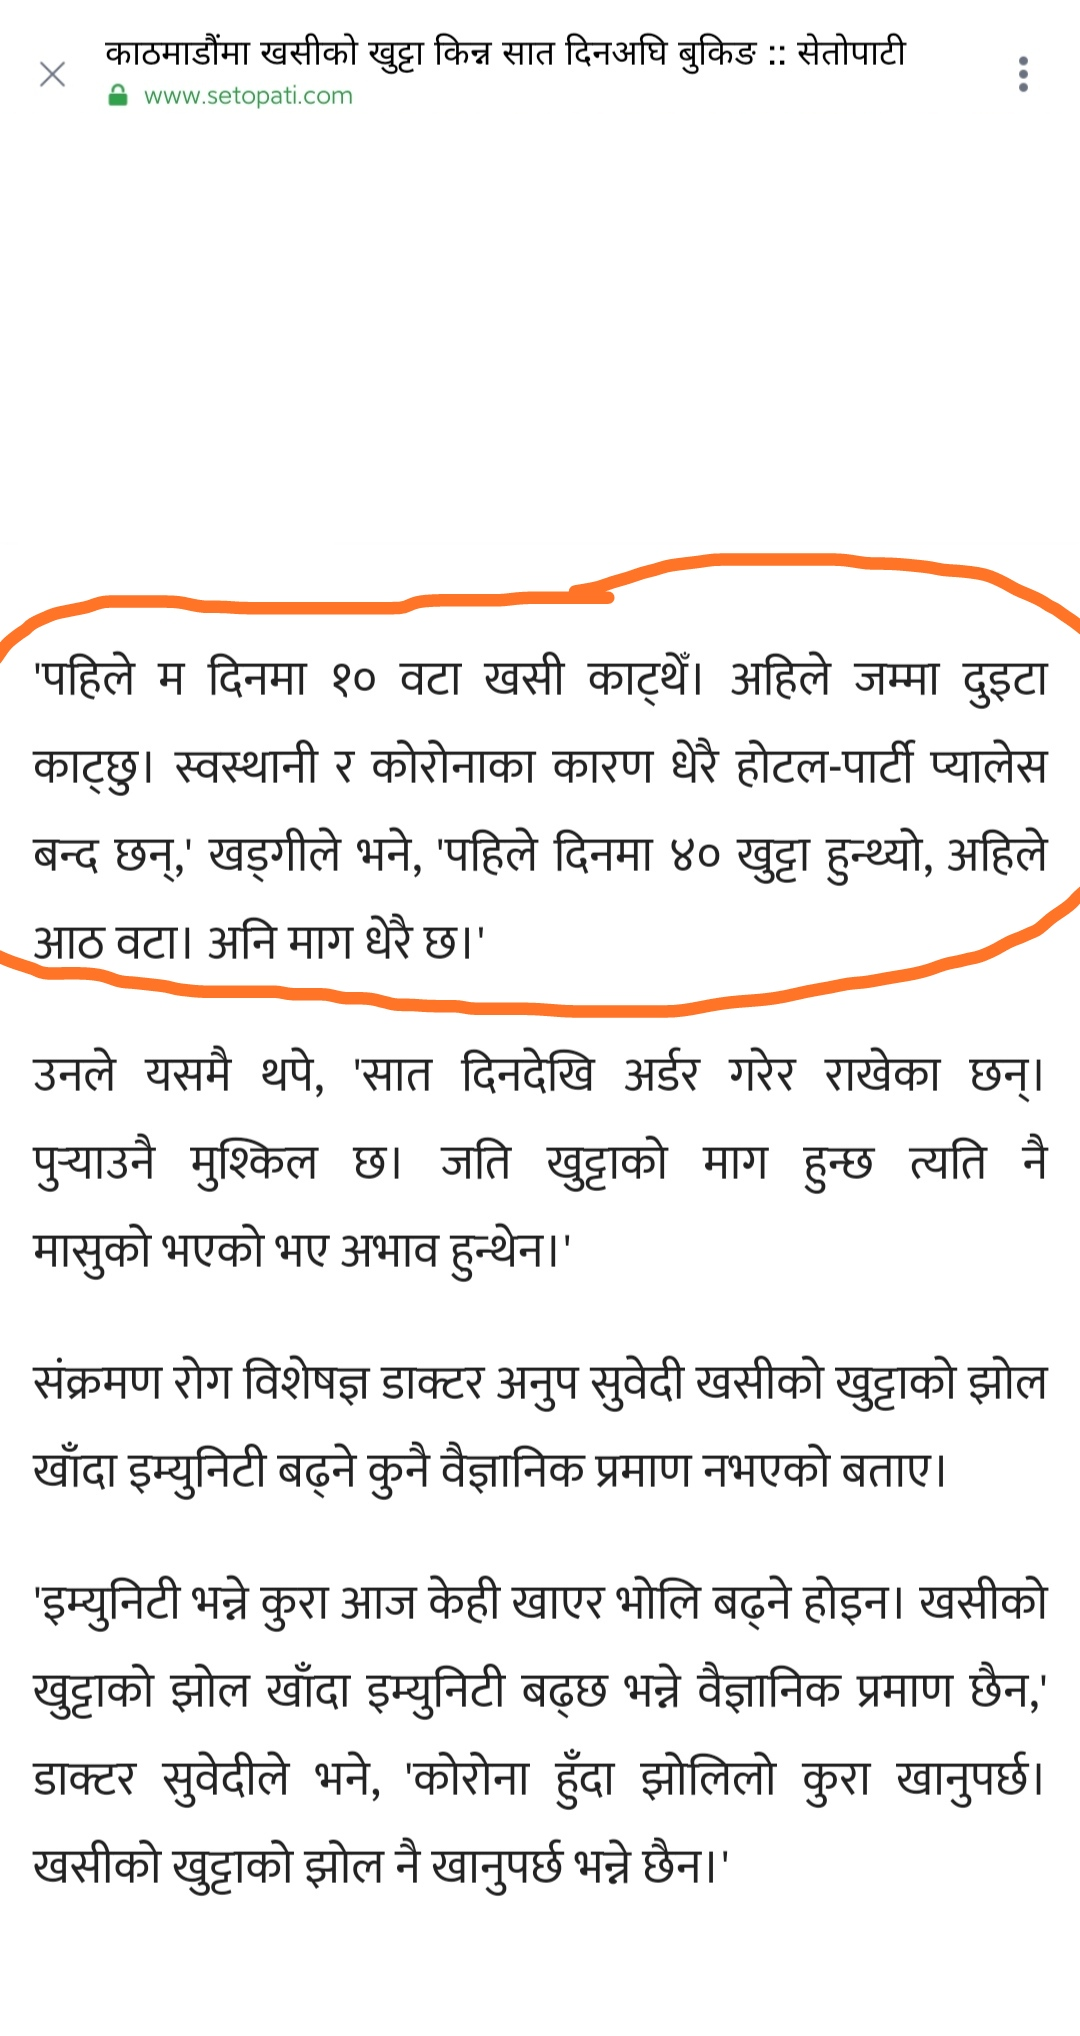
\includegraphics[width=0.6\linewidth]{../images/power_of_legs} 

\end{columns}
\end{frame}

\begin{frame}{Product rule (\(\cap\), \(\land\))}
\protect\hypertarget{product-rule-cap-land}{}
\begin{itemize}
\tightlist
\item
  The possible outcomes from rolling two dice follow the product rule
  because the outcome on one die is independent of the other.
\item
  As an example, let us calculate the probability, \(p\), of rolling a
  pair of 4's (\(\large \{\epsdice{4}, \epsdice{4}\}\)). The probability
  of a \(\large \epsdice{4}\) on one die is 1/6 because the die has six
  sides and only one side carries the number 4.
\item
  This probability is written as follows
\end{itemize}

\[
p ({\large \epsdice{4}}) = \frac{1}{6}
\]

\begin{itemize}
\tightlist
\item
  Therefore, with the use of the product rule, the probability of a 4
  appearing on both dice (\(\large \{\epsdice{4}, \epsdice{4}\}\)) is
  1/6 × 1/6 = 1/36, which is written
\end{itemize}

\[
p (\epsdice{4} \text{ and } \epsdice{4}) = \frac{1}{6} \times \frac{1}{6} = \frac{1}{36}
\]
\end{frame}

\begin{frame}{}
\protect\hypertarget{section}{}
\begin{center}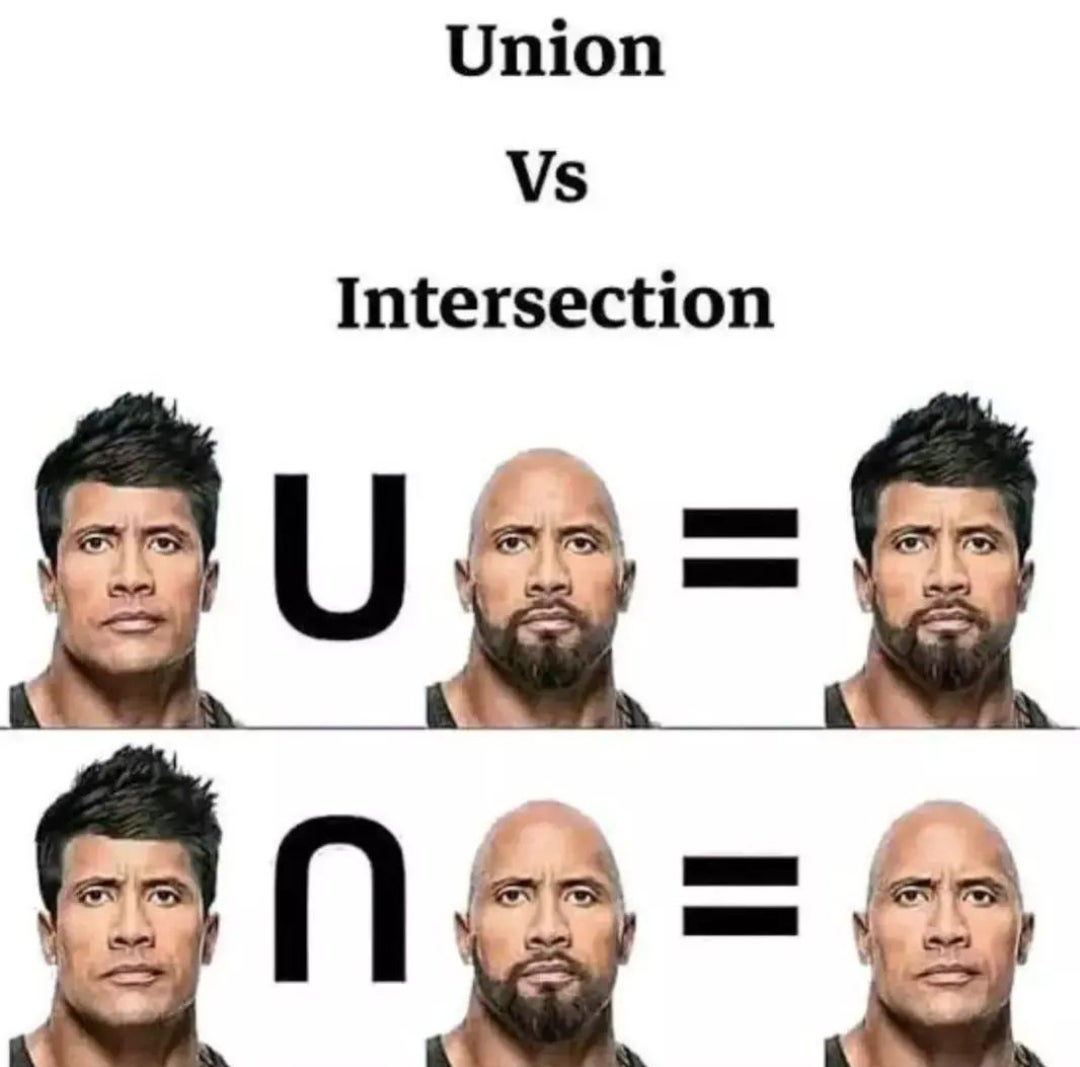
\includegraphics[width=0.45\linewidth]{../images/sum_versus_product} \end{center}
\end{frame}

\begin{frame}{Sum rule (\(\cup\), \(\lor\))}
\protect\hypertarget{sum-rule-cup-lor}{}
\begin{itemize}
\tightlist
\item
  We have already calculated that the probability of
  \(\{\epsdice{4}, \epsdice{4}\}\) is 1/36; clearly, with the use of the
  same type of calculation, the probability of
  \(\{\epsdice{5}, \epsdice{5}\}\) will be the same, or 1/36. Now we can
  calculate the probability of \textbf{either}
  \(\{\epsdice{4}, \epsdice{4}\}\) \textbf{or}
  \(\{\epsdice{5}, \epsdice{5}\}\).
\item
  Because these outcomes are mutually exclusive, the sum rule can be
  used to tell us that the answer is 1/36 + 1/36, which is 1/18. This
  probability can be written as follows:
\end{itemize}

\[
p(\{\epsdice{4}, \epsdice{4}\} \lor \{\epsdice{5}, \epsdice{5}\}) = \frac{1}{36} + \frac{1}{36} = \frac{1}{18}
\]
\end{frame}

\hypertarget{using-large-chi2-test-on-monohybrid-and-dihybrid-ratios}{%
\section{\texorpdfstring{Using \(\Large \chi^2\) test on monohybrid and
dihybrid
ratios}{Using \textbackslash Large \textbackslash chi\^{}2 test on monohybrid and dihybrid ratios}}\label{using-large-chi2-test-on-monohybrid-and-dihybrid-ratios}}

\begin{frame}{Checking observation against expectation}
\protect\hypertarget{checking-observation-against-expectation}{}
\small

\begin{itemize}
\tightlist
\item
  Often the question is whether the obtained results are close to an
  expected ratio, although it is not identical to.
\item
  A statistical test (\(\chi^2\)) checks the observation against
  expectation.
\item
  The general situation is one in which observed results are compared
  with those predicted by a hypothesis.
\item
  In a simple genetic example, suppose you have bred a plant that you
  hypothesize on the basis of a preceding analysis to be a heterozygote,
  A/a.
\item
  To test this hypothesis, you cross this heterozygote with a tester of
  genotype a/a and count the numbers of phenotypes with genotypes A/−
  and a/a in the progeny. Then, you must assess whether the numbers that
  you obtain constitute the expected 1 : 1 ratio.
\item
  If there is a close match, then the hypothesis is deemed consistent
  with the result, whereas if there is a poor match, the hypothesis is
  rejected.
\item
  As part of this process, a judgment has to be made about whether the
  observed numbers are close enough to those expected.
\item
  The \(\chi^2\) test is simply a way of quantifying the various
  deviations expected by chance if a hypothesis is true.
\end{itemize}
\end{frame}

\begin{frame}{Probabilistic testing of data}
\protect\hypertarget{probabilistic-testing-of-data}{}
\begin{itemize}
\tightlist
\item
  We can model this idea with a barrelful of equal numbers of red and
  white marbles. If we blindly remove samples of 100 marbles, on the
  basis of chance we would expect samples to show small deviations such
  as 52 red : 48 white quite commonly and to show larger deviations such
  as 60 red : 40 white less commonly. Even 100 red marbles is a possible
  outcome, at a very low probability of
  \(\left(\frac{1}{2}\right)^{100}\) .
\item
  However, if any result is possible at some level of probability even
  if the hypothesis is true, how can we ever reject a hypothesis? A
  general scientific convention is that a hypothesis will be rejected as
  false if there is a probability of less than 5 percent of observing a
  deviation from expectations at least as large as the one actually
  observed. The implication is that, although results this far from
  expectations are expected 5 percent of the time even when the
  hypothesis is true, we will mistakenly reject the hypothesis in only 5
  percent of cases and we are willing to take this chance of error.
\end{itemize}
\end{frame}

\begin{frame}{Problem 1: Dihybrid testcross ratio}
\protect\hypertarget{problem-1-dihybrid-testcross-ratio}{}
\small

\begin{itemize}
\tightlist
\item
  Consider a general dihybrid testcross, in which it is not known if the
  genes are linked or not: A/a.B/b x a/a.b/b
\item
  If there is \emph{no} linkage, that is, the genes assort
  independently, we have seen that the following phenotypic proportions
  are expected in progeny:
\end{itemize}

\begin{table}
\centering\begingroup\fontsize{6}{8}\selectfont

\begin{tabular}{lr}
\toprule
Phenotype & Proportion\\
\midrule
AB & 0.25\\
Ab & 0.25\\
aB & 0.25\\
ab & 0.25\\
\bottomrule
\end{tabular}
\endgroup{}
\end{table}
\end{frame}

\begin{frame}{}
\protect\hypertarget{section-1}{}
\begin{itemize}
\tightlist
\item
  A cross of this type was made and the following phenotypes obtained in
  a progeny sample of 200.
\end{itemize}

\begin{table}
\centering\begingroup\fontsize{6}{8}\selectfont

\begin{tabular}{lr}
\toprule
Phenotype & Count\\
\midrule
AB & 60\\
Ab & 37\\
aB & 41\\
ab & 62\\
\bottomrule
\end{tabular}
\endgroup{}
\end{table}
\end{frame}

\begin{frame}{Solution 1: Dihybrid testcross ratio}
\protect\hypertarget{solution-1-dihybrid-testcross-ratio}{}
\begin{itemize}
\tightlist
\item
  There is clearly a deviation from the prediction of no linkage which
  would have given the progeny numbers 50:50:50:50.
\item
  The results suggest that the dihybrid was a cis configuration of
  linked genes, A B / a b, because the progeny A B and a b are in the
  majority.
\item
  The recombinant frequency would be \(\frac{37 + 41}{200} = 39\%\), or
  39 m.u.
\item
  However, we know that chance deviations can provide results that
  resemble those produced by genetic processes; hence we, need the
  \(\chi^2\) test to help calculate the probability of a chance
  deviation of this magnitude form a 1:1:1:1 ratio.
\end{itemize}
\end{frame}

\begin{frame}{}
\protect\hypertarget{section-2}{}
\begin{itemize}
\tightlist
\item
  The test statisic \(\chi^2\) is obtained by:
\end{itemize}

\[
\chi^2 = \frac{\left[\sum|observed-expected|-\frac{1}{2}\right]^2}{expected}
\]

\begin{itemize}
\tightlist
\item
  First, let us examine the allele ratios for both loci. These are
  97:103 for A:a, and - 101:99 for B:b. Such numbers are close to the
  1:1 allele ratios expected from mendel's first law, so skewed allele
  ratios cannot be responsible for the quite large deviations from the
  expected numbers of progenies.
\end{itemize}
\end{frame}

\begin{frame}{}
\protect\hypertarget{section-3}{}
\begin{itemize}
\tightlist
\item
  We must apply the \(\chi^2\) analysis to test a hypothesis of no
  linkage. If that hypothesis is rejected, we can infer linkage. (Why
  can't we test a hypothesis of linkage directly ?)
\end{itemize}

\begin{table}

\caption{\label{tab:chi-sqrt-linkage}Chi-square calculations for the hypothesis that the observations of four phenotypic classes is obtained due to no linkage between loci A and B.}
\centering
\resizebox{\linewidth}{!}{
\fontsize{5}{7}\selectfont
\begin{tabular}[t]{lllllr}
\toprule
  & AB & Ab & aB & ab & Totals\\
\midrule
Observed & 60 & 37 & 41 & 62 & 200.0\\
Expected & $\frac{1}{4}\times 200 = 50$ & $\frac{1}{4}\times 200 = 50$ & $\frac{1}{4}\times 200 = 50$ & $\frac{1}{4}\times 200 = 50$ & 200.0\\
Observed - Expected & 10 & -13 & -9 & 12 & \\
$|Observed-Expected|^2$ & 100 & 169 & 81 & 144 & \\
$\left (|Observed-Expected| \right)^2/Expected$ & 2 & 3.38 & 1.62 & 2.88 & \\
\addlinespace
$\chi^2$ &  &  &  &  & 9.9\\
\bottomrule
\end{tabular}}
\end{table}
\end{frame}

\begin{frame}{How I want my P-values vs How they came to be}
\protect\hypertarget{how-i-want-my-p-values-vs-how-they-came-to-be}{}

\includegraphics[width=0.6\linewidth]{../images/my_p_values}
\end{frame}

\begin{frame}{}
\protect\hypertarget{section-4}{}
\begin{table}

\caption{\label{tab:chi-sqrt-values}The probabilities of exceeding different chi-square values for degrees of freedom from 1 to 50 when the expected hypothesis is true}
\centering
\fontsize{5}{7}\selectfont
\begin{tabular}[t]{lrrrr|>{}rrrrrr}
\toprule
  & 0.005 & 0.01 & 0.025 & 0.05 & 0.1 & 0.9 & 0.95 & 0.975 & 0.99 & 0.995\\
\midrule
\cellcolor{gray!6}{1} & \cellcolor{gray!6}{7.9} & \cellcolor{gray!6}{6.6} & \cellcolor{gray!6}{5.0} & \cellcolor{gray!6}{3.8} & \cellcolor{gray!6}{2.7} & \cellcolor{gray!6}{0.02} & \cellcolor{gray!6}{0.00} & \cellcolor{gray!6}{0.00} & \cellcolor{gray!6}{0.00} & \cellcolor{gray!6}{0.00}\\
2 & 10.6 & 9.2 & 7.4 & 6.0 & 4.6 & 0.21 & 0.10 & 0.05 & 0.02 & 0.01\\
\cellcolor{gray!6}{3} & \cellcolor{gray!6}{12.8} & \cellcolor{gray!6}{11.3} & \cellcolor{gray!6}{9.3} & \cellcolor{gray!6}{7.8} & \cellcolor{gray!6}{6.2} & \cellcolor{gray!6}{0.58} & \cellcolor{gray!6}{0.35} & \cellcolor{gray!6}{0.22} & \cellcolor{gray!6}{0.11} & \cellcolor{gray!6}{0.07}\\
4 & 14.9 & 13.3 & 11.1 & 9.5 & 7.8 & 1.06 & 0.71 & 0.48 & 0.30 & 0.21\\
\cellcolor{gray!6}{5} & \cellcolor{gray!6}{16.8} & \cellcolor{gray!6}{15.1} & \cellcolor{gray!6}{12.8} & \cellcolor{gray!6}{11.1} & \cellcolor{gray!6}{9.2} & \cellcolor{gray!6}{1.61} & \cellcolor{gray!6}{1.15} & \cellcolor{gray!6}{0.83} & \cellcolor{gray!6}{0.55} & \cellcolor{gray!6}{0.41}\\
\addlinespace
6 & 18.6 & 16.8 & 14.4 & 12.6 & 10.6 & 2.20 & 1.64 & 1.24 & 0.87 & 0.68\\
\cellcolor{gray!6}{7} & \cellcolor{gray!6}{20.3} & \cellcolor{gray!6}{18.5} & \cellcolor{gray!6}{16.0} & \cellcolor{gray!6}{14.1} & \cellcolor{gray!6}{12.0} & \cellcolor{gray!6}{2.83} & \cellcolor{gray!6}{2.17} & \cellcolor{gray!6}{1.69} & \cellcolor{gray!6}{1.24} & \cellcolor{gray!6}{0.99}\\
8 & 21.9 & 20.1 & 17.5 & 15.5 & 13.4 & 3.49 & 2.73 & 2.18 & 1.65 & 1.34\\
\cellcolor{gray!6}{9} & \cellcolor{gray!6}{23.6} & \cellcolor{gray!6}{21.7} & \cellcolor{gray!6}{19.0} & \cellcolor{gray!6}{16.9} & \cellcolor{gray!6}{14.7} & \cellcolor{gray!6}{4.17} & \cellcolor{gray!6}{3.33} & \cellcolor{gray!6}{2.70} & \cellcolor{gray!6}{2.09} & \cellcolor{gray!6}{1.73}\\
10 & 25.2 & 23.2 & 20.5 & 18.3 & 16.0 & 4.87 & 3.94 & 3.25 & 2.56 & 2.16\\
\addlinespace
\cellcolor{gray!6}{11} & \cellcolor{gray!6}{26.8} & \cellcolor{gray!6}{24.7} & \cellcolor{gray!6}{21.9} & \cellcolor{gray!6}{19.7} & \cellcolor{gray!6}{17.3} & \cellcolor{gray!6}{5.58} & \cellcolor{gray!6}{4.57} & \cellcolor{gray!6}{3.82} & \cellcolor{gray!6}{3.05} & \cellcolor{gray!6}{2.60}\\
12 & 28.3 & 26.2 & 23.3 & 21.0 & 18.6 & 6.30 & 5.23 & 4.40 & 3.57 & 3.07\\
\cellcolor{gray!6}{13} & \cellcolor{gray!6}{29.8} & \cellcolor{gray!6}{27.7} & \cellcolor{gray!6}{24.7} & \cellcolor{gray!6}{22.4} & \cellcolor{gray!6}{19.8} & \cellcolor{gray!6}{7.04} & \cellcolor{gray!6}{5.89} & \cellcolor{gray!6}{5.01} & \cellcolor{gray!6}{4.11} & \cellcolor{gray!6}{3.57}\\
14 & 31.3 & 29.1 & 26.1 & 23.7 & 21.1 & 7.79 & 6.57 & 5.63 & 4.66 & 4.07\\
\cellcolor{gray!6}{15} & \cellcolor{gray!6}{32.8} & \cellcolor{gray!6}{30.6} & \cellcolor{gray!6}{27.5} & \cellcolor{gray!6}{25.0} & \cellcolor{gray!6}{22.3} & \cellcolor{gray!6}{8.55} & \cellcolor{gray!6}{7.26} & \cellcolor{gray!6}{6.26} & \cellcolor{gray!6}{5.23} & \cellcolor{gray!6}{4.60}\\
\addlinespace
16 & 34.3 & 32.0 & 28.9 & 26.3 & 23.5 & 9.31 & 7.96 & 6.91 & 5.81 & 5.14\\
\cellcolor{gray!6}{17} & \cellcolor{gray!6}{35.7} & \cellcolor{gray!6}{33.4} & \cellcolor{gray!6}{30.2} & \cellcolor{gray!6}{27.6} & \cellcolor{gray!6}{24.8} & \cellcolor{gray!6}{10.09} & \cellcolor{gray!6}{8.67} & \cellcolor{gray!6}{7.56} & \cellcolor{gray!6}{6.41} & \cellcolor{gray!6}{5.70}\\
18 & 37.2 & 34.8 & 31.5 & 28.9 & 26.0 & 10.86 & 9.39 & 8.23 & 7.01 & 6.26\\
\cellcolor{gray!6}{19} & \cellcolor{gray!6}{38.6} & \cellcolor{gray!6}{36.2} & \cellcolor{gray!6}{32.9} & \cellcolor{gray!6}{30.1} & \cellcolor{gray!6}{27.2} & \cellcolor{gray!6}{11.65} & \cellcolor{gray!6}{10.12} & \cellcolor{gray!6}{8.91} & \cellcolor{gray!6}{7.63} & \cellcolor{gray!6}{6.84}\\
20 & 40.0 & 37.6 & 34.2 & 31.4 & 28.4 & 12.44 & 10.85 & 9.59 & 8.26 & 7.43\\
\addlinespace
\cellcolor{gray!6}{25} & \cellcolor{gray!6}{46.9} & \cellcolor{gray!6}{44.3} & \cellcolor{gray!6}{40.6} & \cellcolor{gray!6}{37.6} & \cellcolor{gray!6}{34.4} & \cellcolor{gray!6}{16.47} & \cellcolor{gray!6}{14.61} & \cellcolor{gray!6}{13.12} & \cellcolor{gray!6}{11.52} & \cellcolor{gray!6}{10.52}\\
30 & 53.7 & 50.9 & 47.0 & 43.8 & 40.3 & 20.60 & 18.49 & 16.79 & 14.95 & 13.79\\
\cellcolor{gray!6}{35} & \cellcolor{gray!6}{60.3} & \cellcolor{gray!6}{57.3} & \cellcolor{gray!6}{53.2} & \cellcolor{gray!6}{49.8} & \cellcolor{gray!6}{46.1} & \cellcolor{gray!6}{24.80} & \cellcolor{gray!6}{22.47} & \cellcolor{gray!6}{20.57} & \cellcolor{gray!6}{18.51} & \cellcolor{gray!6}{17.19}\\
40 & 66.8 & 63.7 & 59.3 & 55.8 & 51.8 & 29.05 & 26.51 & 24.43 & 22.16 & 20.71\\
\cellcolor{gray!6}{50} & \cellcolor{gray!6}{79.5} & \cellcolor{gray!6}{76.2} & \cellcolor{gray!6}{71.4} & \cellcolor{gray!6}{67.5} & \cellcolor{gray!6}{63.2} & \cellcolor{gray!6}{37.69} & \cellcolor{gray!6}{34.76} & \cellcolor{gray!6}{32.36} & \cellcolor{gray!6}{29.71} & \cellcolor{gray!6}{27.99}\\
\addlinespace
100 & 140.2 & 135.8 & 129.6 & 124.3 & 118.5 & 82.36 & 77.93 & 74.22 & 70.06 & 67.33\\
\bottomrule
\end{tabular}
\end{table}
\end{frame}

\begin{frame}{}
\protect\hypertarget{section-5}{}
\begin{itemize}
\tightlist
\item
  Since there are four genotypic classes, we must use 4-1 = 3 degrees of
  freedom.
\item
  Consulting the \(\chi^2\) table, we see our values of 9.88 and 3 df
  give a p value of \textasciitilde0.025, or 2.5\%.
\item
  This is less than the standard cut-off value of 5 percent, so we can
  reject the hypothesis of no linkage.
\item
  Hence, we are left with the conclusion that the genes are very likely
  linked, approximately 39 m.u. apart.
\end{itemize}
\end{frame}

\begin{frame}{Interpreting p-values}
\protect\hypertarget{interpreting-p-values}{}
\begin{center}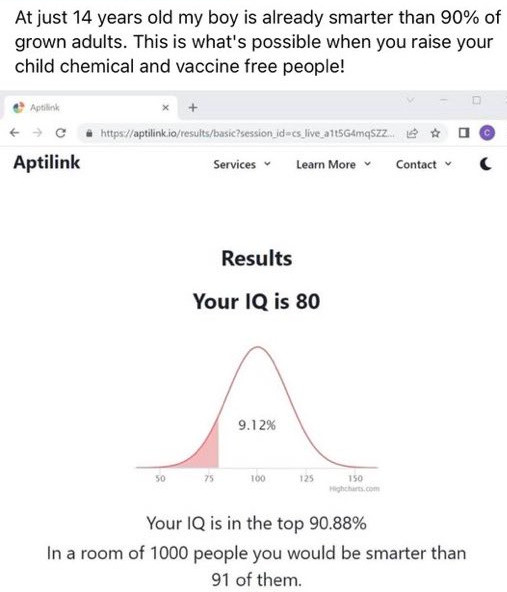
\includegraphics[width=0.4\linewidth]{../images/interpreting_pvalues} \end{center}
\end{frame}

\hypertarget{binomial-expansion}{%
\section{Binomial expansion}\label{binomial-expansion}}

\begin{frame}{}
\protect\hypertarget{section-6}{}
\begin{itemize}
\tightlist
\item
  The set of terms, along with their coefficients, obtained by expanding
  the general binomial \((a + b)^n\) is known as binomial expansion.
\item
  Expansion involves:

  \begin{itemize}
  \tightlist
  \item
    Determination of various terms of the expansion
  \item
    Determination of coefficients of the expansion
  \end{itemize}
\item
  Simplification of \((a + b)^n\) yields following expansion:
\end{itemize}

\[
(a + b)^n = a^n + a^{n-1}b^1 + a^{n-2}b^2 + .... + a^1b^{n-1} + b^n
\]

\begin{itemize}
\tightlist
\item
  The coefficient for a term can be calculated by the following general
  formula:
\end{itemize}

\[
\text{Coefficient} = \frac{n!}{s! t!}
\]

\begin{itemize}
\tightlist
\item
  Where, n = index of binomial, s = index of a in the given term and t =
  index of b in the term.
\item
  It is applicable to those events in which the number of mutually
  exclusive events is two.
\end{itemize}
\end{frame}

\begin{frame}{Problem}
\protect\hypertarget{problem}{}
If 12 people are to be divided into 3 committee of respective sizes, 3,
4 and 5 how many divisions are possible ?

Solution:

A total of \ensuremath{2.77\times 10^{4}} divisions possible.
\end{frame}

\begin{frame}{Problem}
\protect\hypertarget{problem-1}{}
Five male and four female plants are to be arranged in a single row for
a breeding experiment. To ensure breeding, no two male plants can be
next to one another. How many arrangements are possible ?

Solution:

Since there are 5 males and 4 females and there can be no adjacent
males, the plants must alternate between male and female starting with a
male. The number of ordered arrangements of the 5 male plants in the odd
positions is given by \(P_5 = 5!\). Similarly, the number of ordered
arrangements of the 4 female plants in the even positions is given by
\(P_4 = 4!\). Therefore, using the Fundamental Principle of Counting,
the total number of possible arrangements is \(5! \times 4! = 2880\).
\end{frame}

\begin{frame}{Problem}
\protect\hypertarget{problem-2}{}
If 5 coins are tossed together, determine the probability of getting

\begin{enumerate}
\tightlist
\item
  3H and 2T
\item
  At least 3H
\item
  More than 3H
\item
  Less than 3H
\item
  Not more than 3H
\end{enumerate}
\end{frame}

\begin{frame}{Solution}
\protect\hypertarget{solution}{}
Let \(a\) represent probability of turning head (\(P(H) = \frac{1}{2}\))
and \(b\) represent the probability of turning tail
(\(P(T) = \frac{1}{2}\)), then, Binomial expansion can be used to mimic
all 5 tosses.

\[
(a + b)^5 = a^5 + 5a^4b + 10 a^3 b^2 + 10 a^2 b^3 + 5 ab^4 + b^5
\]

Now,

\begin{enumerate}
\tightlist
\item
  Probability(P) of 3H and 2T is given by \(\mathrm{3^{rd}}\) term,
  which is: \(10 a^3 b^2\) equals \(\frac{5}{16}\).
\item
  Probabilities of having (3H or 4H or 5H)
\item
  Probabilities of having (4H or 5H)
\item
  Probabilities of having (1H or 2H)
\item
  Probabilities of having (1H or 2H or 3H)
\end{enumerate}
\end{frame}

\begin{frame}{Problem}
\protect\hypertarget{problem-3}{}
Two heterozygous brown-eyed (Bb) individuals have five children. What is
the probability that two of the couple's five children will have blue
eye ?
\end{frame}

\begin{frame}{Solution}
\protect\hypertarget{solution-1}{}
Applying binomial expansion

\begin{enumerate}
\tightlist
\item
  Calculate individual probabilities (Using punnet square)
\end{enumerate}

\[
\begin{aligned}
P_{(\text{blue eyes})} &= p = \frac{1}{4} \\
P_{(\text{brown eyes})} &= q = \frac{3}{4}
\end{aligned}
\]

\begin{enumerate}
\setcounter{enumi}{1}
\tightlist
\item
  Determine the number of events
\end{enumerate}

\[
\begin{aligned}
n &= \text{total number of children} = 5 \\
x &= \text{total number of blue-eyed children} = 2
\end{aligned}
\]

\begin{enumerate}
\setcounter{enumi}{2}
\tightlist
\item
  Substituting the values in the following binomial equation, \(2^{nd}\)
  term (\(\frac{n!}{s! t!} p^2 q^3\)) and its coefficient gives the
  probability of having two children with blue eyes. That is,
\end{enumerate}

\[
P = \frac{5!}{2! \times 3!} \left(\frac{1}{4}\right)^2 \left(\frac{3}{4}\right)^3 = 0.26
\]

This yields that 26\% of the time, a heterozygote couples' five of the
children will contain two with blue eyes and three with brown eyes.
\end{frame}

\begin{frame}{Problem}
\protect\hypertarget{problem-4}{}
In a family with 5 children, what is the probability that it has 3 boys
and 2 girls among them.
\end{frame}

\begin{frame}{Solution}
\protect\hypertarget{solution-2}{}
Let us assume the probability of having a boy child as \(p\) = 0.5, and
the probability of having a girl child as \(q\) = 0.5. Now the combined
probability of having, among 5 children, 3 boys and 2 girls can
determined by following term of the \((p + q)^5\) binomial expansion.

\[
p^3q^{5-3} = p^3q^{2} = \left(\frac{1}{2}\right)^3 \times \left(\frac{1}{2}\right)^2
\] This has the following coefficient: \(5\choose{3}\)

The probability is, therefore, computed as: 0.31.
\end{frame}

\hypertarget{bibliography}{%
\section{Bibliography}\label{bibliography}}

\begin{frame}{Reading materials}
\protect\hypertarget{reading-materials}{}
For numerical analysis using \(\chi^2\) test, See pp 96 of
\textcite{griffiths2015introduction}.
\end{frame}


  \begin{frame}[allowframebreaks]{}
  \bibliographytrue
  \printbibliography[heading=none]
  \end{frame}


\end{document}
